% Déclaration du type de document (report, book, paper, etc...)
\documentclass[a4paper]{IEEEtran} 
 
% Package pour avoir Latex en français
\usepackage[utf8]{inputenc}
\usepackage[T1]{fontenc}
 
% Quelques packages utiles
\usepackage{listings} % Pour afficher des listings de programmes
\usepackage{graphicx} % Pour afficher des figures
\usepackage{amsthm}   % Pour créer des théorèmes et des définitions
\usepackage{amsmath}
\usepackage{microtype} % Optical margins FTW
\usepackage{url}
\usepackage{booktabs} % Allows the use of \toprule, \midrule and \bottomrule in tables for horizontal lines
\usepackage{siunitx}
\usepackage{floatrow}
\usepackage{caption}
\usepackage{subcaption}
\usepackage{mhchem}
\usepackage[acronym,smallcaps]{glossaries}

\author{Antoine Albertelli\\{a.albertelli@cvra.ch}}
\title{Asynchronous Dead Reckoning Algorithm}

\begin{document}
\maketitle

\section{Conventions}
\begin{figure}[h]
    \begin{center}
        \includegraphics[width=0.8\textwidth]{table}
        \caption{Coordinate system of the robot on the Eurobot table}
        \label{fig:coordinates}
    \end{center}
\end{figure}

The robot has a global coordinate system on the game table (fig. \ref{fig:coordinates}).
The coordinate system is in a direct base.
It is expressed in standard units (\si{\meter} and \si{\radian}).
It doesn't change when changing team color.

The input of the algorithm are the following:
\begin{itemize}
    \item $\Delta_L$ and $\Delta_R$ are the left and right position difference in encoder ticks.
    \item $T$ is the track (distance between the wheels) of the robot in \si{\meter}.
    \item $N$ is the number of encoder ticks per meter.
    \item $\lambda = \frac{R_L}{R_R}$ is the correction factor to account for manufacturing differences between both wheels.
\end{itemize}

\section{Update algorithm}
The base idea of the algorithm is to apply standard dead reckoning formulas but asynchronously, but using the assumption that only the wheel we are updating moved.
That means if we just received $\Delta_L$, we assume that $\Delta_R$ is zero.

\begin{figure}[h]
    \begin{center}
        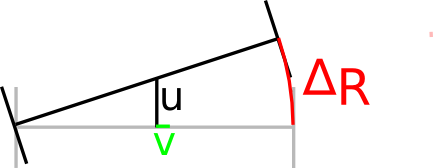
\includegraphics[width=0.4\textwidth]{algorithm.png}
        \caption{Visual explanation of the algorithm}
    \end{center}
\end{figure}

We start by computing the difference in heading $\Delta_\theta$:

\begin{equation}
    \Delta_\theta = \frac{\Delta_R - \Delta_L}{T}
\end{equation}

Then we can compute the robot movement :

\begin{equation}
    \begin{pmatrix}
        u\\v
    \end{pmatrix}  
    =
    \frac{T}{2}
    \begin{pmatrix}
        \sin \Delta_\theta\\1 - \cos \Delta_\theta
    \end{pmatrix}
    \approx
    \frac{T}{2}
    \begin{pmatrix}
        \Delta_\theta\\ 0
    \end{pmatrix}
\end{equation}

We will then transpose those displacement vector in the global space:

\begin{equation}
    \begin{pmatrix}
        \Delta_x\\\Delta_y
    \end{pmatrix}
    =
    \begin{pmatrix}
        \cos\theta \\-\sin\theta
    \end{pmatrix}
    u 
\end{equation}

Finally, integrate the change into the robot position:
\begin{equation}
    \begin{pmatrix}
        x_{k+1}\\
        y_{k+1}\\
        \theta_{k+1}
    \end{pmatrix}
    =
    \begin{pmatrix}
        x_{k}\\
        y_{k}\\
        \theta_{k}
    \end{pmatrix}
    +
    \begin{pmatrix}
        \Delta_x\\\Delta_y\\\Delta_\theta
    \end{pmatrix}
\end{equation}


\section{Accounting for mechanical tolerances}
In the previous sections we supposed that the two measuring wheels were perfectly identical, with the same tick to meter ratio.
However, in the real world, manufacturing tolerances are not perfect and wheel diameters can vary quite a lot.
Using the ISO 2768-f specification on a \SI{40}{\milli\meter} yields a maximum tolerance of $\pm \SI{0.2}{\milli\meter}$.
This means that between both wheels the maximum relative error is $\frac{\Delta_R}{R} = \frac{2 \cdot 0.2}{40} = 1\% $.

How does this error translate into robot trajectory ?
Well when the robot thinks it is doing a straight line, it will actually be turning in a slight circle.

Each will will run on a cirlcle of radius $R$.
The distance between the wheels is fixed so :
\begin{equation}
    R_1 - R_2 = T
\end{equation}

The robot turned of a given angle $\alpha$ so :
\begin{equation}
    R_1 \alpha = \lambda R_2 \alpha
\end{equation}

Therefore:
\begin{equation}
    (T + R_2) \alpha = \lambda R_2 \alpha
\end{equation}

And finally we got the radius of the trajectory :
\begin{equation}
    R = T \left(\frac{1}{\lambda - 1}  + \frac{1}{2}\right)
\end{equation}

Plugging reasonable parameters for Eurobot ($\lambda=1+0.1\%$, $T = \SI{0.2}{\meter}$), we obtain a radius $R = \SI{300}{\meter}$. 
Such a big radius might seem indistinguishable from a straight line, but this is not the case.
To show this, let's compute the lateral deviation on a full table crossing (\SI{2.5}{\meter}):
\begin{equation}
    \Delta_x = \left( 1 - \cos \frac{2.5}{300} \right) \cdot \SI{300}{\meter} \approx \SI{1}{\centi\meter}
\end{equation}

This shows that compensating for manufacturing tolerances is critical for a good odometry.






\end{document}
